\documentclass[12pt]{article}

\usepackage{amsfonts, amsmath, amssymb}
\usepackage[top=20mm, bottom=20mm, left=28mm, right=28mm]{geometry}
\usepackage{graphicx} % Required for including pictures
\usepackage{float} % Allows putting an [H] in \begin{figure} to specify the exact location of the figure
\usepackage{xcolor,pict2e}
\usepackage{enumitem}

\usepackage{algorithm}
\usepackage{algorithmicx}
\usepackage{algpseudocode}
\usepackage{listings}

\definecolor{backcolour}{rgb}{0.95,0.95,0.92}
\definecolor{codegreen}{rgb}{0,0.6,0}

% Define a custom style
\lstdefinestyle{myStyle}{
    backgroundcolor=\color{backcolour},   
    commentstyle=\itshape\color{codegreen},
	identifierstyle=\color{blue},
    basicstyle=\ttfamily\footnotesize,
    breakatwhitespace=false,
    breaklines=true,
    keepspaces=true,
    frame=none,
    numbers=none,
    showspaces=false,
    showstringspaces=false,
    showtabs=false,
    tabsize=4,
}

\lstset{style=myStyle}



\DeclareMathSizes{14pt}{12pt}{12pt}{12pt} 

\linespread{1.35} % Line spacing

\renewcommand{\thefootnote}{\fnsymbol{footnote}}

% \renewcommand{\algorithmicrequire}{\textbf{Input:}}  % Use Input in the format of Algorithm
\renewcommand{\algorithmicensure}{\textbf{Outcome:}} % Use Output in the format of Algorithm






\begin{document}

\title{\fontsize{18}{24} \bf Approximate solutions of integro-differential equations by piecewise 3rd Bezier functions and conjugate gradient method}
\author{\normalsize Shou-Jyun Zou\thanks{sgzou2000@gmail.com}}
\date{\small \today}


\maketitle


\begin{abstract}
	This is an algorithm for finding the numerical solution of the general (2nd order) integro-differential equation by the piecewise polynomial (3rd Bezier) functions.
	The main improvements here are the consideration of the piecewise 3rd Bezier functions with $\mathcal{C}^1$ continuity and the use of the conjugate gradient method to find the approximate solution of integro-differential equations.
\end{abstract}


\tableofcontents





%%%%%%%%%%%%%%%%%%%%%%%%%%%%%%%%%%%%%%%%%%%%%%%%%%%%%%%%%%%%%%%
\section{Bezier functions}
%%%%%%%%%%%%%%%%%%%%%%%%%%%%%%%%%%%%%%%%%%%%%%%%%%%%%%%%%%%%%%%





A \textbf{3rd order Bezier function} can be written as
%
\begin{align*}
	X(t) \;=\; & P_{0} \left( \frac{t_{e}-t}{t_{e}-t_{s}} \right)^3 + 3 P_{1} \left( \frac{t_{e}-t}{t_{e}-t_{s}} \right)^2 \left( \frac{t-t_{s}}{t_{e}-t_{s}} \right) + 3 P_{2} \left( \frac{t_{e}-t}{t_{e}-t_{s}} \right) \left( \frac{t-t_{s}}{t_{e}-t_{s}} \right)^2 + P_{3} \left( \frac{t-t_{s}}{t_{e}-t_{s}} \right)^3 \\
	\;=\; & \sum_{j=0}^3 P_j B_j(t,t_{s},t_{e}) \qquad \textrm{ for $t\in [t_{s}, t_{e})$}
\end{align*}
%
where $t_{s},t_{e}$ are the constants of the start point and end point in the domain space, $P_0,P_1,P_2,P_3$ are the constant vectors (or scalars) in the target space called control points, and
%
\begin{align*}
	B_j(t,t_{s},t_{e}) \;=\; \binom{3}{i} \left( \frac{t_{e} - t}{t_{e} - t_{s}} \right)^{3-i} \left( \frac{t - t_{s}}{t_{e} - t_{s}} \right)^{i}
\end{align*}
%
are known as the Bernstein basis polynomials of degree $3$.


A \textbf{piecewise 3rd Bezier function} can be written as
%
\begin{align*}
	X(t) \;=\; \left\{ \begin{array}{l l}
		\sum_{j=0}^3 P_j B_j(t,t_{0s},t_{0e}) & \textrm{ for } t\in [t_{0s},t_{0e}) \\
		\sum_{j=0}^3 P_{3+j} B_j(t,t_{1s},t_{1e}) & \textrm{ for } t\in [t_{1s}=t_{0e},t_{1e}) \\
		\qquad \vdots \\
		\sum_{j=0}^3 P_{3k+j} B_j(t,t_{ks},t_{ke}) & \textrm{ for } t\in [t_{ks}=t_{(k-1)e},t_{ke})
	\end{array} \right. 
\end{align*}
%
It is a series of Bezier functions joined end to end, and the last point of one curve coincides with the starting point of the next piece.






%%%%%%%%%%%%%%%%%%%%%%%%%%%%%%%%%%%%%%%%%%%%%%%%%%%%%%%%%%%%%%%
\section{The idea of an approximate solution using Bezier functions}
%%%%%%%%%%%%%%%%%%%%%%%%%%%%%%%%%%%%%%%%%%%%%%%%%%%%%%%%%%%%%%%





%%%%%%%%%%%%%%%%%%%%%%%%%%%%%%%%%%%%%%%%%%%%%%%%%%%%%%%%%%%%%%%
\subsection{Example : $\ddot{X}(t) = 2 t^5$}
%%%%%%%%%%%%%%%%%%%%%%%%%%%%%%%%%%%%%%%%%%%%%%%%%%%%%%%%%%%%%%%


Let consider the differential equation system
%
\begin{align*}
	\left\{ \begin{array}{c}
		\ddot{X}(t) = 2 t^5 \qquad t \in [t_s=0,\, t_e=1]\\
		\textrm{initial condition: } \quad \dot{X}(0) = 3 \;,\; X(0) = 2 \\
	\end{array} \right.
\end{align*}
%
Suppose an approximate solution X(t) is written as a 3rd order Bezier polynomial
%
\begin{align*}
	X(t) \;=\; & P_{0} \left( \frac{t_{e}-t}{t_{e}-t_{e}} \right)^3 + 3 P_{1} \left( \frac{t_{e}-t}{t_{e}-t_{e}} \right)^2 \left( \frac{t-t_{s}}{t_{e}-t_{s}} \right) + 3 P_{2} \left( \frac{t_{e}-t}{t_{e}-t_{e}} \right) \left( \frac{t-t_{s}}{t_{e}-t_{s}} \right)^2 + P_{3} \left( \frac{t-t_{s}}{t_{e}-t_{s}} \right)^3
\end{align*}
%
Substitute the function back into the equation, the problem now becomes an algebraic problem
%
\begin{align*}
	\ddot{X}(t) \;=\; & \left( 6P_0 - 12P_1 + 6P_2 \right) + \left( -6P_0 + 18P_1 - 18P_2 + 6P_3 \right) t \;\approx\; 2 t^5 \quad \textrm{for $t\in[0,1]$} \\
	\dot{X}(0) \;=\; & - 3P_0 + 3P_1 \;=\; 3 \qquad,\qquad X(0) \;=\; P_0 \;=\; 2
\end{align*}
%
We define the residual $R(P_i)$ of the system as 
%
\begin{align}
	R(P_i) \;=\; \int \left( \ddot{X}(t)-2t^5 \right)^2 dt + \lambda_1 (X(0)-2)^2 + \lambda_2 (\dot{X}(0)-3)^2
\end{align}
%
where $\lambda_1,\lambda_2$ are two large numerical constants.
The residual $R(P_i)$ is a non-negative function, the minimal condition of this function can give an approximate solution of the differential equation system.


\textbf{To find the minimal condition of the residual function is an optimized problem}, one can use the gradient descent method, that we can use the gradient $\frac{\partial R(P_i)}{\partial P_i}$ to find the direction of the minimal point.
Here, we use the \textbf{conjugate gradient method}, that is more efficient in most cases of numerical computation.\cite{Shewchuk:1994}


Note, $\frac{\partial R(P_i)}{\partial P_2}$ can be estimated in this way:
%
\begin{align*}
	\frac{\partial R(P_i)}{\partial P_2} & \;=\; \lim_{P'_2\to P_2} \frac{1}{P'_2 - P_2}\left[ \int \left( \ddot{X'}(t)-2t^5 \right)^2 dt - \int \left( \ddot{X}(t)-2t^5 \right)^2 dt \right]  \\
	& \;=\; \int \frac{\partial \left( \ddot{X}(t)-2t^5 \right)^2}{\partial \ddot{X}} \frac{\partial \ddot{X}}{\partial P_2} dt \\
	& \;=\; \int \frac{\partial R(X)}{\partial \ddot{X}(t)} \frac{\partial \ddot{X}}{\partial P_2} dt
\end{align*}





%%%%%%%%%%%%%%%%%%%%%%%%%%%%%%%%%%%%%%%%%%%%%%%%%%%%%%%%%%%%%%%
\subsection{$\mathcal{C}^1$ piecewise 3rd Bezier function}
%%%%%%%%%%%%%%%%%%%%%%%%%%%%%%%%%%%%%%%%%%%%%%%%%%%%%%%%%%%%%%%


Piecewise polynomial function approximation is needed for more complex problems.

The piecewise 3rd Bezier functions is 
%
\begin{footnotesize}
	\begin{align*}
		X(t) = \left\{ \begin{array}{c l}
			P_{0} \left( \frac{t_{0e}-t}{t_{0e}-t_{0s}} \right)^3 + 3 P_{1} \left( \frac{t_{0e}-t}{t_{0e}-t_{0s}} \right)^2 \left( \frac{t-t_{0s}}{t_{0e}-t_{0s}} \right) + 3 P_{2} \left( \frac{t_{0e}-t}{t_{0e}-t_{0s}} \right) \left( \frac{t-t_{0s}}{t_{0e}-t_{0s}} \right)^2 + P_{3} \left( \frac{t-t_{0s}}{t_{0e}-t_{0s}} \right)^3 &, \; t\in [t_{0s}, t_{0e}) \\
			P_{3} \left( \frac{t_{1e}-t}{t_{1e}-t_{1s}} \right)^3 + 3 P_{4} \left( \frac{t_{1e}-t}{t_{1e}-t_{1s}} \right)^2 \left( \frac{t-t_{1s}}{t_{1e}-t_{1s}} \right) + 3 P_{5} \left( \frac{t_{1e}-t}{t_{1e}-t_{1s}} \right) \left( \frac{t-t_{0s}}{t_{1e}-t_{1s}} \right)^2 + P_{6} \left( \frac{t-t_{1s}}{t_{1e}-t_{1s}} \right)^3 &, \; t\in [t_{1s}, t_{1e}) \\
			\qquad \vdots \\
			P_{3k} \left( \frac{t_{ke}-t}{t_{ke}-t_{ks}} \right)^3 + 3 P_{3k+1} \left( \frac{t_{ke}-t}{t_{ke}-t_{ks}} \right)^2 \left( \frac{t-t_{ks}}{t_{ke}-t_{ks}} \right) + 3 P_{3k+2} \left( \frac{t_{ke}-t}{t_{ke}-t_{ks}} \right) \left( \frac{t-t_{ks}}{t_{ke}-t_{ks}} \right)^2 + P_{3k+3} \left( \frac{t-t_{ks}}{t_{ke}-t_{ks}} \right)^3 &, \; t\in [t_{ks}, t_{ke}] \\
		\end{array} \right.
	\end{align*}
\end{footnotesize}
%
where $t_{ks}=t_{(k-1)e}$.
If we consider all the control points $P_1,P_2,\dots, P_{3k+3}$ are all independent and use the gradient $\frac{\partial R(P_i)}{\partial P_i}$ to find the minimal condition.
In most cases, we will get the wrong answer and most of them have non-differentiable points in the joined points $P_3, P_6, \dots, P_{3k}$.


So, we imply $C^1$ conditions $\lim_{\epsilon\to 0}\frac{d X(t+\epsilon)}{dt} |_{t=t_{i\,e}} = \lim_{\epsilon\to 0}\frac{d X(t-\epsilon)}{dt} |_{t=t_{i\,e}}$, and it implies
%
\begin{align}
	P_{3i+1} \;=\; 2P_{3i} - P_{3i-1}
\end{align}
%
So, the real independent control points are $P_0,P_1,P_2,P_3,P_5,P_6,P_8,P_9,\dots,P_{3k-1},P_{3k},\dots$, and $P_{3i+1}$ ($i\ge 1$) are determined by $P_{3i}, P_{3i-1}$.


We can directly apply the relation $P_{3i+1} = 2P_{3i} - P_{3i-1}$, and say $\frac{d R}{d P_{3i-1}} = \int \frac{\partial R(X)}{\partial X(t)} \frac{\partial X}{\partial P_{3i+1}} \frac{\partial P_{3i+1}}{\partial P_{3i-1}} dt + \frac{\partial R}{\partial P_{3i-1}} = - \int \frac{\partial R(X)}{\partial X(t)} \frac{\partial X}{\partial P_{3i+1}} dt + \frac{\partial R}{\partial P_{3i-1}}$.
But the convergence usually is bad.
This is because $P_{3i-1}$ and $P_{3i}$ both modify $P_{3i+1}$, so part of their effects are reduced.
\textbf{The better linked action in the calculation:}
In the iteration viewpoint, a better situation is that, $P_{3i-1}$ involves $P_{3i}$, and later $P_{3i}$ involves $P_{3i+1}$.
So, all of them can be modified sequentially.
To realize the relation and to reflect the differentiable continuity, we consider the differential of $P_{3i-1}$ with the correction from $P_{3i}$:
%
\begin{align*}
	\frac{d R}{d P_{3i-1}} & \;=\; \int \frac{\partial R(X)}{\partial X(t)} \frac{\partial X}{\partial P_{3i}}\frac{\partial P_{3i}}{\partial P_{3i-1}} dt + \frac{\partial R}{\partial P_{3i-1}} \\
	& \;=\; \int \frac{\partial R(X)}{\partial X(t)} \left( \frac{t-t_{is}}{t_{ie}-t_{is}} \right)^3 \frac{1}{2} dt + \frac{\partial R}{\partial P_{3i-1}}
\end{align*}
%
This means that the variation of $P_{3i-1}$ also involves $P_{3i}$ but not changes other control points.
See the following sub-figure (b).
So, when we vary $P_{3i-1}$, we also need to modify $P_{3i}$ with the differentiable continuity condition.
There are no problem for $P_{3i}$ and $P_{3i+1}$, we can use the original formula: $\frac{d R}{d P_{3i}} \;=\; 2\int \frac{\partial R(X)}{\partial X(t)}\frac{\partial X}{\partial P_{3i+1}} dt + \frac{\partial R}{\partial P_{3i}}$.
See the following sub-figure (c).
We don't change $P_{3i+1}$ directly, but use $P_{3i+1} = 2P_{3i} - P_{3i-1}$ to elemeliminate all the $P_{3i+1}$ ($i\ge 1$) control points.
Now, we can get the gradient vectors $\frac{d R}{d P_j}$ without the $P_{3i+1}$ ($i\ge 1$) control points.
And using the gradient vectors, we can sequentially modify the control points $P_{i}$ (without $P_{3i+1}$ ($i\ge 1$)) and preserve the differentiable continuity condition.
%
\begin{figure}[H]
	\centering
	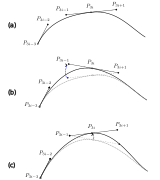
\includegraphics[width=0.5\linewidth]{move.jpg}
	\caption{The schematic diagram for the sequence movement.}
\end{figure}


Usually the residual depends on the derivative $R(X,\dot{X},\ddot{X})$, the argument is the same as above and here we should take 
%
\begin{align*}
	\frac{d R}{d P_{3i-1}} & \;=\; \int \left( \frac{\partial R(X)}{\partial X(t)} \frac{\partial X}{\partial P_{3i}} + \frac{\partial R(X)}{\partial \dot{X}(t)} \frac{\partial \dot{X}}{\partial P_{3i}} + \dots \right)\frac{\partial P_{3i}}{\partial P_{3i-1}} dt \\
	& \qquad \qquad + \int \left( \frac{\partial R(X)}{\partial X(t)} \frac{\partial X}{\partial P_{3i-1}} + \frac{\partial R(X)}{\partial \dot{X}(t)} \frac{\partial \dot{X}}{\partial P_{3i-1}} + \dots \right) dt \\
	& \;=\; \int \left\{ \left( \frac{\partial R(X)}{\partial X(t)} \frac{\partial X}{\partial P_{3i}} + \frac{\partial R(X)}{\partial \dot{X}(t)} \frac{\partial \dot{X}}{\partial P_{3i}} + \dots \right)\frac{1}{2} + \left( \frac{\partial R(X)}{\partial X(t)} \frac{\partial X}{\partial P_{3i-1}} + \frac{\partial R(X)}{\partial \dot{X}(t)} \frac{\partial \dot{X}}{\partial P_{3i-1}} + \dots \right) \right\} dt
\end{align*}





%%%%%%%%%%%%%%%%%%%%%%%%%%%%%%%%%%%%%%%%%%%%%%%%%%%%%%%%%%%%%%%
\subsection{Multi-variable function cases}
%%%%%%%%%%%%%%%%%%%%%%%%%%%%%%%%%%%%%%%%%%%%%%%%%%%%%%%%%%%%%%%


The multi-variable function of the Bezier function is written as
%
\begin{align}
	X(\tau,\sigma) \;=\; \sum_{i=0}^3 \sum_{j=0}^3 B_i(\tau) B_j(\sigma) P_{ij}
\end{align}
%
where $P_{ij}$ are the control points, and
%
\begin{align*}
	B_i(\tau) \;=\; \binom{3}{i} \left( \frac{\tau_e - \tau}{\tau_e - \tau_s} \right)^{3-i} \left( \frac{\tau - \tau_s}{\tau_e - \tau_s} \right)^{i} \quad,\quad B_j(\sigma) \;=\; \binom{3}{j} \left( \frac{\sigma_e - \sigma}{\sigma_e - \sigma_s} \right)^{3-j} \left( \frac{\sigma - \sigma_s}{\sigma_e - \sigma_s} \right)^{j}
\end{align*}
%
are the Bernstein basis polynomials.


Most of the idea in the previous discussion can be applied to the multi-variable cases.
But \textbf{the differentiable continuity in different direction need to be noted here}.
In implementation, we will deform $P_{3i}$, $P_{3i+2}$ via the gradient of the residual function and use the differentiable continuity condition to modify $P_{3i+1}$.
However, in multi-variable case, the differentiable continuity condition can not be guaranteed.
For example, $P_{(3i-1)\,(3j+1)},P_{(3i)\,(3j+1)}$ set the position of $P_{(3i+1)\,(3j+1)}$ via the differentiable continuity condition in the direction of $i$ parameter.
And, by the similar way in the direction of the $j$ parameter, $P_{(3i+1)\,(3j-1)},P_{(3i+1)\,(3j)}$ also try to set the position of $P_{(3i+1)\,(3j+1)}$.
Usually, the later change will break the first setting of the differentiable continuity condition.
So, in multi-variable case, we need use $P_{(3i+1)...}$ and go back to modify $P_{(3i)...}$ in all directions to make sure the differentiable continuity.





%%%%%%%%%%%%%%%%%%%%%%%%%%%%%%%%%%%%%%%%%%%%%%%%%%%%%%%%%%%%%%%
\section{Pseudocode for optimizing control point state}
%%%%%%%%%%%%%%%%%%%%%%%%%%%%%%%%%%%%%%%%%%%%%%%%%%%%%%%%%%%%%%%


\begin{algorithm}[H]
	\renewcommand{\thealgorithm}{}
	\caption{Finding the control point state of the minimal residual by the conjugate gradient method.}
	\begin{algorithmic}[1]
		\Require 
		(a). The arbitrary piecewise 3rd Bezier function $X(t)=\sum P_i B_i(t)$. \qquad\qquad  (b). The system residual $R(X,\dot{X},\ddot{X})$ and the gradient $\frac{\partial R(X)}{\partial X(t)}\frac{\partial X}{\partial P_i}$.
		\Ensure
		The minimized residual $R$ value and the associated control point state $\{P_i\}$. \vspace{2mm}
		\Repeat
			\State compute the residual $r=R(\{P_i\})$;
        	\State estimate the gradient $\frac{\partial R}{\partial P_i}$ for all $P_i$;	\Comment{by the proposal of \S 2.2}
			\State use conjugate gradient to get all deformation vectors $\Delta P_i$;
			\While{$r$ can be minimized as $r'$}
				\State \texttt{SmoothDeform($s \{\Delta P_i\}$)};		\Comment{by the proposal of \S 2.2}
				\State new residual $r'=R(\{P_i + s \Delta P_i\})$;		\Comment{$s$ is deformation scale}
		  	\EndWhile
			\If{allowed deformation scale $s$ too small}
			  \State slightly perturbate $P_i$ and restart conjugate gradient;
			\EndIf
		\Until{($r$ is small enough)} \\
		\Return $R$ and $\{P_i\}$;
	\end{algorithmic}
\end{algorithm}
%
In implementation, we usually find that the residual can be further minimized if we slightly perturbate $P_i$ and restart conjugate gradient algorithm.
So, we add the step 10 in the pseudocode.






%%%%%%%%%%%%%%%%%%%%%%%%%%%%%%%%%%%%%%%%%%%%%%%%%%%%%%%%%%%%%%%
\section{Numerical test}
%%%%%%%%%%%%%%%%%%%%%%%%%%%%%%%%%%%%%%%%%%%%%%%%%%%%%%%%%%%%%%%


find the soliton wave configuration.





%%%%%%%%%%%%%%%%%%%%%%%%%%%%%%%%%%%%%%%%%%%%%%%%%%%%%%%%%%%%%%%
\subsection{Lorenz system}
%%%%%%%%%%%%%%%%%%%%%%%%%%%%%%%%%%%%%%%%%%%%%%%%%%%%%%%%%%%%%%%


\begin{align*}
	\frac{dx}{dt} \;=\; & \sigma(y-x) \\
	\frac{dy}{dt} \;=\; & x(\rho-z) - y \\
	\frac{dz}{dt} \;=\; & xy-\beta z
\end{align*}
%
The initial data and parameters here are $x(0)=10,y(0)=10,z(0)=10$ and $\sigma=10,\rho=28,\beta=8/3$.
If we directly write down the residual function for this 3 dimension 1 variable differential system as $R = \int \left\{ (\dot{x}-\sigma(y-x))^2 + (\dot{y}-x(\rho-z)+y)^2 + (\dot{z}-xy+\beta z)^2 \right\} dt + 10000((x(0)-10)^2+(y(0)-10)^2+(z(0)-10)^2)$.
We can get the approximate solution in the short time interval $t\in [0,0.2]$.
But the longer time interval cases are not easy to converge.

\begin{figure}[H]
	\centering
	\includegraphics[width=1.0\linewidth]{../lorenz_system/data/lorenz_system_ex.png}
	\caption{Here, the time interval is $t\in [0,0.2]$ and the number of control points is 37}
\end{figure}





%%%%%%%%%%%%%%%%%%%%%%%%%%%%%%%%%%%%%%%%%%%%%%%%%%%%%%%%%%%%%%%
\subsection{O'Hara knot energy}
%%%%%%%%%%%%%%%%%%%%%%%%%%%%%%%%%%%%%%%%%%%%%%%%%%%%%%%%%%%%%%%





%%%%%%%%%%%%%%%%%%%%%%%%%%%%%%%%%%%%%%%%%%%%%%%%%%%%%%%%%%%%%%%
\subsubsection{O'Hara knot energy integral}
%%%%%%%%%%%%%%%%%%%%%%%%%%%%%%%%%%%%%%%%%%%%%%%%%%%%%%%%%%%%%%%


Let $\gamma(u)$ be a curve in the Euclidean 3-space $\mathbb{R}^{3}$.
The O'Hara knot energy formula is
%
\begin{align*}
	E(\gamma) \;=\; \int\int \left\{ \frac{1}{|\gamma(u)-\gamma(v)|^2} - \frac{1}{D(\gamma(u),\gamma(v))^2} \right\}|\dot{\gamma}(u)||\dot{\gamma}(v)| du\, dv
\end{align*}
%
where $D(\gamma (u),\gamma (v))$ is the shortest arc distance between $\gamma (u)$ and $\gamma (v)$ on the curve. 
(So $D(\gamma (u),\gamma (v)) = |\int_u^v |\dot{\gamma}(t)|dt|$.
If $\gamma$ is a circle with total length $L$, then $D(\gamma (u),\gamma (v)) = \min\{ |\int_u^v |\dot{\gamma}(t)|dt|,\, L - |\int_u^v |\dot{\gamma}(t)|dt| \}$ )


Here, we want to use our algorithm to find the minimal energy of a isotopic knot.
The first thing is to generate a knot by using our Bezier function:
%
\begin{lstlisting}[language=c++]
	coordinate inipt;      // the initial point of the curve
    inipt.coord.push_back(0.2);
    inipt.coord.push_back(0.2);
    inipt.coord.push_back(0.2);

    std::map<std::array<int,4>, coordinate> fixPts;  // The key of the dictionary must be array<int,4> which corresponds to P_{ijkl} of Bezier function X(x,y,z,w)=P_{ijkl}B_i(x)B_j(y)B_k(z)B_l(w). And we only use the first index of array<int,4> for one dimensional curve.
    fixPts[{{0,0,0,0}}] = inipt;
    fixPts[{{15,0,0,0}}] = inipt;

    std::array<double,2> intvl = {{0.0, 1.0}};
    std::vector<std::array<double,2>> interval;
    interval.push_back(intvl);	

	std::vector<int> cPtsN = {15}; // the max index of control points in each dimension

	BezierImage curve;
	curve.RandGenerator(cPtsN, fixPts, interval); 
\end{lstlisting}


The in order to implement conjugate gradient optimization, we need to implement the numerical integral of the O'Hara knot energy for our Bezier curve.
In the O'Hara knot energy we need the information $|\dot{\gamma}(u)|$ and $D(\gamma (0),\gamma (u)) = \int_0^u |\dot{\gamma}(t)|dt$, so we record them in the arraies \textsf{tangentLength[]} and \textsf{arcLengthFrom0[]}:
%
\begin{lstlisting}[language=c++]
	t1[0] = img.DomainInterval[0][0];
	for (int i = 0; i < samples[0]+1; i++)
	{
		v = img.DiffBezierMap(t1,0);
		tangentLength[i] = sqrt(VectorLenSquare(v.coord));  // |gamma'(t1)|
		if (i==0) // record arc length from 0 to t1
		{
			arcLengthFrom0[i] = tangentLength[i]*stepGap;
		}
		else
		{
			arcLengthFrom0[i] = arcLengthFrom0[i-1] + tangentLength[i]*stepGap;
		}
		t1[0] = t1[0] + stepGap;
	}
\end{lstlisting}
%
Then the numerical is straightforward
%
\begin{lstlisting}[language=c++]
	t1[0] = img.DomainInterval[0][0];
	t2[0] = img.DomainInterval[0][0];
	for (int i = 0; i < samples[0]+1; i++)
	{
		for (int j = 0; j < samples[0]+1; j++)
		{
			if (i != j & !( i==0 & j == samples[0]) & !( i==samples[0] & j == 0))
			{
				// O'Hara energy integral
				energy = energy + (( 1.0/img.DistanceSquare(t1,t2) ) - ( 1.0/pow(std::min(abs(arcLengthFrom0[i]-arcLengthFrom0[j]),arcLengthFrom0[samples[0]]-abs(arcLengthFrom0[i]-arcLengthFrom0[j])), 2) )) * tangentLength[i] * tangentLength[j];                        
			}

			if ((i==0 & j==samples[0]) || (j ==0 && i==samples[0]))
			{
				energy = energy + 1.0E+20*img.DistanceSquare(t1,t2);  // inforce the start point and end point can not change too much.
			}

			t2[0] = t2[0] + stepGap;
		}
		t1[0] = t1[0] + stepGap;
		t2[0] = img.DomainInterval[0][0];
	}
\end{lstlisting}





%%%%%%%%%%%%%%%%%%%%%%%%%%%%%%%%%%%%%%%%%%%%%%%%%%%%%%%%%%%%%%%
\subsubsection{Gradient of O'Hara knot energy integral for control points}
%%%%%%%%%%%%%%%%%%%%%%%%%%%%%%%%%%%%%%%%%%%%%%%%%%%%%%%%%%%%%%%


With $\vec{\gamma}(u) = \sum \vec{P}_i B_i(u)$ (later we ignore the vector symbol), $E(\gamma) = \int\int \left\{ \frac{1}{|\gamma(u)-\gamma(v)|^2} - \frac{1}{D(\gamma(u),\gamma(v))^2} \right\}|\dot{\gamma}(u)||\dot{\gamma}(v)| du\, dv$, we want to calculate $\frac{\partial E(\gamma)}{\partial P_i}$.
We should estimate each term
%
\begin{align*}
	\frac{\partial}{\partial P_i} \left( \frac{1}{|\gamma(u)-\gamma(v)|^2} \right) \;=\; & \frac{\partial}{\partial P_i} \left( \frac{1}{(\gamma(u)-\gamma(v))\cdot (\gamma(u)-\gamma(v))} \right) \\
	\;=\; & - \frac{2(\gamma(u)-\gamma(v))(B_i(u)-B_i(v))}{|\gamma(u)-\gamma(v)|^4}
\end{align*}
%
\begin{align*}
	\frac{\partial}{\partial P_i} \left( |\dot{\gamma}(u)| \right) \;=\; & \frac{\partial}{\partial P_i} \left( \sqrt{\dot{\gamma}(u)\cdot\dot{\gamma}(u)} \right) \\
	\;=\; & \frac{\dot{\gamma}(u)\dot{B}_i(u)}{|\dot{\gamma}(u)|}
\end{align*}
%
\begin{align*}
	\frac{\partial}{\partial P_i} \left( \frac{1}{D(\gamma(u),\gamma(v))^2} \right) \;=\; & \frac{\partial}{\partial P_i} \left( \frac{1}{(\int_u^v |\dot{\gamma}(t)|dt)^2} \right) \\
	\;=\; & - \frac{2\int_u^v\frac{(\dot{\gamma}(t))\dot{B}(t)}{|\dot{\gamma}(t)|}dt}{(\int_u^v |\dot{\gamma}(t)|dt)^3}
\end{align*}
%
As $D(\gamma (0),\gamma (u)) = \int_0^u |\dot{\gamma}(t)|dt$ are recorded in the array \textsf{arcLengthFrom0[]}, here we need the information $\int_0^u\frac{(\dot{\gamma}(t))\dot{B}(t)}{|\dot{\gamma}(t)|}dt$ and they are recorded in the array \textsf{arcLengthFrom0Derivative[]}.
Because $D(\gamma (u),\gamma (v)) = \min\{ |\int_u^v |\dot{\gamma}(t)|dt|,\, L - |\int_u^v |\dot{\gamma}(t)|dt| \}$, so in the implementation of $\int_u^v\frac{(\dot{\gamma}(t))\dot{B}(t)}{|\dot{\gamma}(t)|}dt$ we estimate them as the following way:
%
\begin{lstlisting}[language=c++]
	if ( abs(arcLengthFrom0[i]-arcLengthFrom0[j]) < arcLengthFrom0[samples[0]]-abs(arcLengthFrom0[i]-arcLengthFrom0[j]) )
	{
		arcLength = abs(arcLengthFrom0[i]-arcLengthFrom0[j]);
		for (int c = 0; c < img.TargetDimeion; c++)
		{
			arcLengthDerivative.coord[c] = copysign(1.0, arcLengthFrom0[i]-arcLengthFrom0[j]) * (arcLengthFrom0Derivative[i].coord[c] - arcLengthFrom0Derivative[j].coord[c]);
		}
	}
	else
	{
		arcLength = arcLengthFrom0[samples[0]]-abs(arcLengthFrom0[i]-arcLengthFrom0[j]);
		for (int c = 0; c < img.TargetDimeion; c++)
		{
			arcLengthDerivative.coord[c] = arcLengthFrom0Derivative[samples[0]].coord[c] - copysign(1.0, arcLengthFrom0[i]-arcLengthFrom0[j])*(arcLengthFrom0Derivative[i].coord[c] - arcLengthFrom0Derivative[j].coord[c]);
		}
	}
\end{lstlisting}
%
where we multiply \textsf{copysign(1.0, arcLengthFrom0[i]-arcLengthFrom0[j])} on \textsf{(arcLengthFrom0Derivative[i].coord[c] - arcLengthFrom0Derivative[j].coord[c])}, because we need the integral order of $\int_u^v\frac{(\dot{\gamma}(t))\dot{B}(t)}{|\dot{\gamma}(t)|}dt$ is always from the point of small arc length to the point of large arc length that is due to the meaning of $D(\gamma (u),\gamma (v)) = \min\{ |\int_u^v |\dot{\gamma}(t)|dt|,\, L - |\int_u^v |\dot{\gamma}(t)|dt| \}$ is positive.


\begin{figure}[H]
	\centering
	\includegraphics[width=1.0\linewidth]{../knot_energy/data/knot_energy_ex.png}
	%\caption{Here, the time interval is $t\in [0,0.2]$ and the number of control points is 37}
\end{figure}





%%%%%%%%%%%%%%%%%%%%%%%%%%%%%%%%%%%%%%%%%%%%%%%%%%%%%%%%%%%%%%%
\subsection{Wave equation}
%%%%%%%%%%%%%%%%%%%%%%%%%%%%%%%%%%%%%%%%%%%%%%%%%%%%%%%%%%%%%%%


\begin{figure}[H]
	\centering
	\includegraphics[width=1.0\linewidth]{../wave_equation/data/wave_equation_ex.png}
	%\caption{Here, the time interval is $t\in [0,0.2]$ and the number of control points is 37}
\end{figure}








\appendix









%%%%%%%%%%%%%%%%%%%%%%%%%%%%%%%%%%%%%%%%%%%%%%%%%%%%%%%%%%%%%%%%%%%%%%%%%%%%%%%%%%%%%%%%%%%%

\begin{thebibliography}{0}
	
	\bibitem{Lewis:2023}
	K~Lewis, T~Matsuura,
	``Bezier Curve Method to Compute Various Meniscus Shapes,''
	ACS Omega, \textbf{8}, issue 17, 15371-15383 (2023)
	DOI: 10.1021/acsomega.3c00620

	\bibitem{Ghomanjani:2012}
	F~Ghomanjani, M.H.~Farahi,
	``The Bezier Control Points Method for Solving Delay Differential Equation,''
	Intelligent Control and Automation, \textbf{3} No.2, 188-196 (2012)
	DOI: 10.4236/ica.2012.32021 

	\bibitem{Ghomanjani:2018}
	F~Ghomanjani, K~Khorram,
	``Approximate solution for quadratic Riccati differential equationFootnote,''
	Journal of Taibah University for Science, \textbf{181}(2), 246-250 (2018)
	DOI: 10.1016/j.jtusci.2015.04.001

	\bibitem{Ghomanjani:2022}
	F~Ghomanjani, S~Noeiaghdam, S~Micula,
	``Application of Transcendental Bernstein Polynomials for Solving Two-Dimensional Fractional Optimal Control Problems,''
	Complexity, \textbf{2022} 1, 4303775 (2022)
	DOI: 10.1155/2022/4303775

	\bibitem{Ghomanjani:2019}
	F~Ghomanjani, S~Shateyi,
	``A new approach for solving Bratu's problem,''
	Demonstratio Mathematica, \textbf{52}, 336-346 (2019)
	DOI: 10.1515/dema-2019-0023

	\bibitem{Ghomanjani:2017}
	F~Ghomanjani, M.H~Farahi, N~Pariz,
	``A new approach for numerical solution of a linear system with distributed delays, Volterra delay-integro-differential equations, and nonlinear Volterra-Fredholm integral equation by Bezier curves,''
	Comp. Appl. Math. \textbf{36}, 1349-1365 (2017)
	DOI: 10.1007/s40314-015-0296-2

	\bibitem{Darehmiraki:2016}
	M~Darehmiraki, M.H~Farahi, S~Effati,
	``A Novel Method to Solve a Class of Distributed Optimal Control Problems Using Bezier Curves,''
	J. Comput. Nonlinear Dynam. \textbf{11}(6), 061008 (2016)
	DOI: 10.1115/1.4033755

	\bibitem{Ghomanjani:2013}
	F~Ghomanjani, A~Kilicman, S~Effati,
	``Numerical Solution for IVP in Volterra Type Linear Integrodifferential Equations System,''
	Abstract and Applied Analysis \textbf{2013}(1), 490689 (2013)
	DOI: 10.1155/2013/490689

	\bibitem{Ghomanjani:2013}
	E~Erkan, S~Yuce,
	``Serret-Frenet Frame and Curvatures of Bezier Curves,''
	Mathematics, \textbf{6}(12), 321 (2018)
	DOI: 10.3390/math6120321

	\bibitem{Beltran:2004}
	J.V.~Beltran, J.~Monterde ,
	``Bezier Solutions of the Wave Equation,''
	Computational Science and Its Applications - ICCSA (2004) Conference paper, 631-640

	\bibitem{Zheng:2004}
	J~Zheng, T.W.~Sederberg, R.W.~Johnson,
	``Least squares methods for solving differential equations using Bezier control points,''
	Applied Numerical Mathematics \textbf{48}(2), 237-252 (2004)
	DOI: 10.1016/j.apnum.2002.01.001

	\bibitem{Bhatti:2007}
	M.I.~Bhatti, P.~Bracken,
	``Solutions of differential equations in a Bernstein polynomial basis,''
	Journal of Computational and Applied Mathematics  \textbf{205}, Issue 1, 272-280 (2007)
	DOI: 10.1016/j.cam.2006.05.002

	\bibitem{Basirat:2013}
	B.~Basirat, M.A.~ Shahdadi,
	``Numerical Solution of Nonlinear Integro-Differential Equations with Initial Conditions by Bernstein Operational Matrix of Derivative,''
	International Journal of Modern Nonlinear Theory and Application \textbf{2} No.2, 141-149 (2013)
	DOI: 10.4236/ijmnta.2013.22018

	\bibitem{Venkataraman:2007}
	P.~Venkataraman, J.G.~Michopoulos,
	``Explicit Solutions for Nonlinear Partial Differential Equations Using Bezier Functions,''
	International Design Engineering Technical Conferences and Computers and Information in Engineering Conference (2007) 69-80
	DOI: 10.1115/DETC2007-35439

	\bibitem{Ordokhani:2011}
	Y.~Ordokhani, S.~Davaei far,
	``Approximate Solutions of Differential Equations by Using the Bernstein Polynomials,''
	International Scholarly Research Notices \textbf{2011}(1), 787694 (2011)
	DOI: 10.5402/2011/787694

	\bibitem{Bencheikh:2017}
	A.~Bencheikh, L.~Chiter, H.~Abbassi,
	``Bernstein polynomials method for numerical solutions of  integro-differential form of the singular Emden-Fowler initial value problems,''
	Journal of Mathematics and Computer Science \textbf{17}(1), 66-75 (2017)
	DOI: 10.22436/jmcs.017.01.06	
	
	\bibitem{Razvarz:2018}
	S.~Razvarz, R.~Jafari, A.~Gegov ,
	``Solving Partial Differential Equations with Bernstein Neural Networks,''
	Advances in Computational Intelligence Systems Conference paper (2018) 57-70

	\bibitem{Shewchuk:1994}
	J.R.~Shewchuk, 
	``An introduction to the conjugate gradient method without the agonizing pain,''
	(1994)

\end{thebibliography}



\end{document}

